\documentclass{article}

\usepackage{fancyhdr} % Required for custom headers
\usepackage{lastpage} % Required to determine the last page for the footer
\usepackage{extramarks} % Required for headers and footers
\usepackage{graphicx} % Required to insert images
\usepackage{lipsum} % Used for inserting dummy 'Lorem ipsum' text into the template
\usepackage{ulem} % Required for Cross out text
\usepackage{amsmath} % Required for Math Stuff
\usepackage{amsfonts}
\usepackage{enumerate}
%\usepackage[]{algorithm2e}
\usepackage{hyperref}
%\usepackage{qtree}
\usepackage{hyperref}

\usepackage{caption}
\usepackage{subcaption}

% Margins
\topmargin=-0.45in
\evensidemargin=0in
\oddsidemargin=0in
\textwidth=6.5in
\textheight=9.0in
\headsep=0.25in

\linespread{1.1} % Line spacing

%----------------------------------------------------------------------------------------

\begin{document}

\title{Notes on regrasping as an underactuated pivot}
\author{Annie}
\maketitle
%%\vspace{-0.7in}

%----------------------------------------------------------------------------------------
%	Math Commands
%----------------------------------------------------------------------------------------

\providecommand{\abs}[1]{\left\vert#1\right\vert}
\providecommand{\norm}[1]{\left\Vert#1\right\Vert}

\begin{figure}[h!]
  \centering
  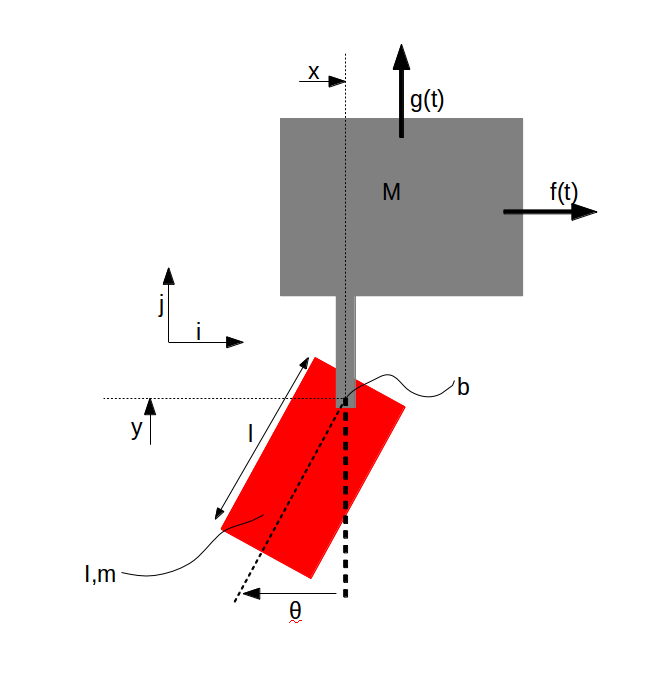
\includegraphics[width=0.75\textwidth]{diagram.png}
  \caption{A rough sketch of the system. The hand is in gray with gripper coming down and the block in red.}
\end{figure}

As a first pass at the problem of pivoting a block into any angle using the dynamics of the system, I am approaching it as an underactuated system where the grasp acts as a pivot joint with a certain rotation damping due to the friction of the grasp, $b$. The block has a mass $m$, moment of inertia about the block's center of mass $I$, and a length $l$. The hand has a mass, $M$ and its can move in the $\hat{i}$ and $\hat{j}$ directions as functions  $f(t)$ and $g(t)$. 

\section{Generalized Coordinate System and Forces}

There are three degrees of freedom here (assuming no motion in the $\hat{k}$ is relevant), which are x,y, and $\theta$. Positive x points to the right, y up, and $\theta$ clockwise measured from the downward position.  
$$
\zeta_j: x,y, \theta
$$
with the variation $\zeta_j: \delta x, \delta y, \delta \theta$

The generalized forces, $\Xi_j$ can be obtained fromt the work where
$$
\delta W = \overset{n}{\underset{i = 1}{\sum}} \mathbf{F_i} \cdot \delta \mathbf{r_i} = \overset{n}{\underset{j = 1}{\sum}} \Xi_j \delta \zeta_j
$$

Nonconservative forces from the inputs $g(t)$ and $f(t)$ and the damping $b$ around the grasp result in,
$$
\delta W = f(t) \delta x + g(t) \delta y - b \dot{\theta}\delta\theta
$$ 
So we get:
$$
\Xi_x = f(t) \\
\Xi_y = g(t) \\
\Xi_{\theta} = -b\dot{\theta}
$$

\section{Kinetic Energy}

The kinetic energy of the hand (the cart in simple cases): 
$$
K_{hand} = \frac{1}{2}M\mathbf{v}^2
$$

Where $M$ is the mass of the hand and v is a planar velocity vector of the hand (lets just assume x,y for now since movement in the same axis as the pivot axis doesnt do anything). \\

The kinetic energy for the block:
$$
K_{block} = \frac{1}{2} m\mathbf{v_c}^2 + \frac{1}{2} I \omega^2
$$

where $v_c$ is the velocity of the center of mass of the block, $m$ is the mass of the block, $I$ is the moment of inertia around the block's center of mass, and $\omega$ is the angular velocity. \\
The position vector can then be written,
$$
\mathbf{r_c} = (x - l\sin(\theta)) \hat{i} + (y - l\cos(\theta)) \hat{j}
$$
$$
\mathbf{v_c} = \frac{d\mathbf{r_c}}{dt} = (\dot{x} - l \cos(\theta)\dot{\theta}) \hat{i} + (\dot{y} + l\sin(\theta)\dot{\theta} \hat{j}
$$

Then, $\omega = \dot{\theta}$ \\
So plugging in we get, 
$$
K_{block} = \frac{1}{2} m (\dot{x}^2 - 2 \dot{x}lcos(\theta)\dot{\theta} + l^2cos^2(\theta)\dot{\theta}^2 + \dot{y}^2 + 2 \dot{y}lsin(\theta)\dot{\theta} + l^2sin^2(\theta)\dot{\theta}^2) + \frac{1}{2} I \dot{\theta}^2
$$
$$
 =  \frac{1}{2} m (\dot{x}^2 - 2 \dot{x}l\cos(\theta)\dot{\theta} + \dot{y}^2 + 2 \dot{y}l\sin(\theta)\dot{\theta} + l^2\dot{\theta}^2) + \frac{1}{2} I \dot{\theta}^2
$$
Then our total kinetic energy is, 
$$
K = K_{hand} + K_{block} = \frac{1}{2} M(\dot{x}^2+\dot{y}^2) + \frac{1}{2} m (\dot{x}^2 - 2 \dot{x}l\cos(\theta)\dot{\theta} + \dot{y}^2 + 2 \dot{y}l\sin(\theta)\dot{\theta} + l^2\dot{\theta}^2) + \frac{1}{2} I \dot{\theta}^2
$$

\section{Potential Energy}

$$
P = -mg(y+l)cos(\theta)
$$

\section{Lagrangian}

Fromt he kinetic and potential energies, the lagrangians is given by
$$
L = K - P
$$
which becomes
$$
L = \frac{1}{2} M(\dot{x}^2+\dot{y}^2) + \frac{1}{2} m (\dot{x}^2 - 2 \dot{x}l\cos(\theta)\dot{\theta} + \dot{y}^2 + 2 \dot{y}l\sin(\theta)\dot{\theta} + l^2\dot{\theta}^2) + \frac{1}{2} I \dot{\theta}^2 + mg(y+l)\cos(\theta)
$$

\subsection{More Lagrange Shit}

The equations for x,
$$
\Xi_x = \frac{d}{dt} (\frac{\partial L}{\partial \dot{x}} ) - \frac{\partial L}{\partial x}
$$
$$
\frac{d}{dt} (M\dot{x} + m\dot{x} - ml\cos(\theta)\dot{\theta}) = f(t) 
$$
$$
(M+m)\ddot{x} - ml\cos(\theta)\ddot{\theta} + ml\sin(\theta)\dot{\theta}^2 = f(t) 
$$

The same for y, 
$$
\Xi_y = \frac{d}{dt} (\frac{\partial L}{\partial \dot{y}} ) - \frac{\partial L}{\partial y}
$$
$$
\frac{d}{dt} (M\dot{y} + m\dot{y} + ml\sin(\theta)\dot{\theta}) - mg\cos(\theta) = g(t) 
$$
$$
(M+m)\ddot{y} + ml\sin(\theta)\ddot{\theta} - ml\cos(\theta)\dot{\theta}^2 - mg\cos(\theta) = g(t)
$$

And for $\theta$,
$$
\Xi_{\theta} = \frac{d}{dt} (\frac{\partial L}{\partial \dot{\theta}} ) - \frac{\partial L}{\partial \theta}
$$
$$
\frac{d}{dt} (-m\dot{x}l\cos(\theta) + m\dot{y}l\sin(\theta) + ml^2\dot{\theta} + I\dot{\theta}) - (ml\dot{x}\sin(\theta)\dot{\theta} + ml\dot{y}\cos(\theta)\dot{\theta} - mg\sin(\theta)) = -b \dot{\theta}
$$
$$
(ml^2 + I)\ddot{\theta} -ml\ddot{x}\cos(\theta)+ml\dot{x}\sin(\theta)\dot{\theta}+ml\ddot{y}\sin(\theta)+ml\dot{y}\cos(\theta)\dot{\theta} - (ml\dot{x}\sin(\theta)\dot{\theta} + ml\dot{y}\cos(\theta)\dot{\theta} - mg\sin(\theta))= -b \dot{\theta}
$$
where $b$ is a rotational damping coefficient around the grasp. \\

Now we have to solve for $f(t)$ (motion in the $\hat{i}$ direction) and $g(t)$ (motion in the $\hat{j}$ direction)

\begin{equation} \label{eq:x}
(M+m)\ddot{x} - ml\cos(\theta)\ddot{\theta} + ml\sin(\theta)\dot{\theta}^2 = f(t) 
\end{equation}
\begin{equation} \label{eq:y}
(M+m)\ddot{y} + ml\sin(\theta)\ddot{\theta} - ml\cos(\theta)\dot{\theta}^2 - mg\cos(\theta) = h(t)
\end{equation}
\begin{equation} \label{eq:theta}
(ml^2 + I)\ddot{\theta} + b \dot{\theta} -ml\ddot{x}\cos(\theta) +ml\ddot{y}\sin(\theta) + mg\sin(\theta)= 0
\end{equation}

\section{Energy Regulation using PFLs}

\subsection{Collocated Partial Feedback Linearization (PFL)}

Our goal is for $\ddot{x} = \ddot{x_d}$ and $\ddot{y} = \ddot{y_d}$. We can solve for $\ddot{\theta}$ using ~\ref{eq:theta}
$$
\ddot{\theta} = \frac{1}{ml^2} (-mgs -mls\ddot{y} +mlc\ddot{x} -b\dot{\theta})
$$
Where $s = \sin(\theta)$ and $c= \cos(\theta)$. \\
\noindent
If we plug this into ~\ref{eq:y} 

$$
(M+m)\ddot{y} + mls(\frac{1}{ml^2} (-mgs -mls\ddot{y} +mlc\ddot{x} -b\dot{\theta})) - mlc\dot{\theta}^2 - mgc = h(t)
$$
$$
(M+m)\ddot{y} + \frac{s}{l} (-mgs -mls\ddot{y} +mlc\ddot{x} -b\dot{\theta}) - mlc\dot{\theta}^2 - mgc = h(t)
$$
$$
\ddot{y} = \frac{1}{M+mc^2} (h(t)+\frac{mgs^2}{l}-msc\ddot{x}+\frac{bs\dot{\theta}}{l}+mlc\dot{\theta}^2+mgc)
$$
Then into ~\ref{eq:x} 
$$
(M+m)\ddot{x} - ml\cos(\theta)\ddot{\theta} + ml\sin(\theta)\dot{\theta}^2 = f(t) 
$$
etc. etc. etc.

\subsection{Energy Regulation}

If $\ddot{x} = \bar{u}$ and $\ddot{y} = \bar{v}$, then 
$$
\ddot{\theta} = \frac{1}{ml^2} (-mgs -mls\bar{v} +mlc\bar{u} -b\dot{\theta})
$$

From before our energy is given by,
$$
E =  \frac{1}{2} ml^2\dot{\theta}^2 -  mg(y+l)c
$$
$$
\dot{E} = ml^2 \dot{\theta}\ddot{\theta} + mg(y+l)s\dot{\theta}
$$
$$
\dot{E} = ml^2 \dot{\theta}(\frac{1}{ml^2} (-mgs -mls\bar{v} +mlc\bar{u} -b\dot{\theta})) + mg(y+l)s\dot{\theta}
$$
$$
\dot{E} = \dot{\theta}(-mgs -mls\bar{v} +mlc\bar{u} -b\dot{\theta}) + mg(y+l)s\dot{\theta}
$$
So to increase the energy, we can chose and $\bar{u}$ and $\bar{v}$ to make this expression positive. For example,

$$
\bar{u} = kmlc\dot{\theta} \bar{E}
$$
$$
\bar{v} = -kmls\dot{\theta} \bar{E} 
$$

Where $\bar{E}$ is the difference between the desired energy and the actual energy.

\subsection{now wat}

We have two problems: we have no feedback for $\dot{\theta}$, and
since our desired energy is not at an equilibrium point, it won't have
zero kinetic energy, so we don't really know what $\bar{E}$ is. \\ \\
\noindent
The first is easier to deal with. If we just put in just enough energy
to get to $\theta$ before it begins decreasing, we will be at zero
velocity at the apex of a path arc at $\theta$. So our $E_d =
mg(y+l)\cos(\theta)$. \\ \\
\noindent 
To handle no feedback (which is inherent in this problem since the
block is always connected at the fingertips where there is no sensing
normally), we can predict what $\theta$ is ideally doing based on the
equations of motion. \\ \\
\noindent
Let's plug our expression for $\ddot{\theta}$ into ~\ref{eq:x} (or we could use ~\ref{eq:y})
$$
\ddot{\theta} = \frac{1}{ml^2} (-mgs -mls\bar{v} +mlc\bar{u} -b\dot{\theta})
$$
We know that $f(t) = \bar{u}$ and that $\ddot{x} = \frac{f(t)}{m} = klc\dot{\theta}$. Similarly for $\ddot{y}$
$$
\ddot{\theta} = \frac{1}{ml^2} (-mgs -mls(-kls\dot{\theta}) +mlc(klc\dot{\theta}) -b\dot{\theta})
$$
$$
\ddot{\theta} = \frac{1}{ml^2} (-mgs +kml^2\dot{\theta} -b\dot{\theta})
$$
\noindent
From ~\ref{eq:x}, $(M+m)\ddot{x} - ml\cos(\theta)\ddot{\theta} + ml\sin(\theta)\dot{\theta}^2 = f(t) $

$$
(M+m)(klc\dot{\theta}) - ml\cos(\theta)(\frac{1}{ml^2} (-mgs +kml^2\dot{\theta} -b\dot{\theta})) + ml\sin(\theta)\dot{\theta}^2 = kmlc\dot{\theta}
$$
\begin{equation} \label{eq:t1}
(M-m)(klc\dot{\theta}) + \frac{cb\dot{\theta}}{l} + \frac{mgsc}{l} + mls\dot{\theta}^2 = 0
\end{equation}
\noindent
From ~\ref{eq:y}, $(M+m)\ddot{y} + ml\sin(\theta)\ddot{\theta} - ml\cos(\theta)\dot{\theta}^2 - mg\cos(\theta) = h(t)$

$$
(M+m)(-kls\dot{\theta}) + ml\sin(\theta)(\frac{1}{ml^2} (-mgs +kml^2\dot{\theta} -b\dot{\theta})) - ml\cos(\theta)\dot{\theta}^2 - mg\cos(\theta) = -kmls\dot{\theta}
$$
\begin{equation} \label{eq:t2}
(m-M)(kls\dot{\theta}) - \frac{bs\dot{\theta}}{l} -\frac{mgs^2}{l} - mlc\dot{\theta}^2 - mgc = 0
\end{equation}
\noindent
To solve for $\theta$ and $\dot{\theta}$, we can multiply ~\ref{eq:t1} by $\cos(\theta)$, ~\ref{eq:t2} by $\sin(\theta)$, and add.

$$
(M-m)(klc^2\dot{\theta}) + \frac{c^2b\dot{\theta}}{l} + \frac{mgsc^2}{l} + mlsc\dot{\theta}^2 = 0
$$
$$
(m-M)(kls^2\dot{\theta}) - \frac{bs^2\dot{\theta}}{l} -\frac{mgs^3}{l} - mlsc\dot{\theta}^2 - mgsc = 0
$$
\noindent
Giving
$$
(M-m)(kl\dot{\theta}) + \frac{b\dot{\theta}}{l} + \frac{mgs}{l} + mgsc = 0
$$
\noindent
Then we can solve for $\dot{\theta}$ and integrate to get $\theta$
$$
\dot{\theta} = \frac{1}{(M-m)kl + \frac{b}{l}}(-mgsc - \frac{mgs}{l})
$$
$$
\theta = \frac{1}{(M-m)kl + \frac{b}{l}} (-\frac{mgc^2}{2} +\frac{mgc}{l})
$$
\noindent
If we substitute these expressions back into our control laws $\bar{u}$ and $\bar{v}$, we get
$$
\bar{u} =  \frac{kml}{(M-m)kl + \frac{b}{l}} * c(-mgsc - \frac{mgs}{l}))
$$
$$
\bar{v} = \frac{-kml}{(M-m)kl + \frac{b}{l}} *  s(-mgsc - \frac{mgs}{l}))
$$

\noindent
Ignoring costants those expressions roughly look like
$$
\bar{u} = \cos(\theta) * (-\sin(\theta)\cos(\theta)-\sin(\theta))
$$
$$
\bar{v} = \sin(\theta) * (-\sin(\theta)\cos(\theta)-\sin(\theta))
$$

\begin{figure}[h!]
  \centering
  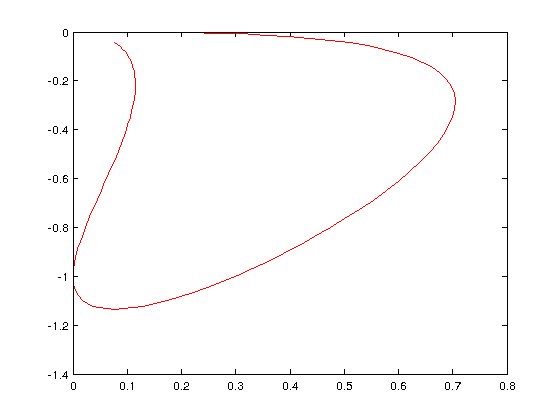
\includegraphics[width=0.75\textwidth]{curve2.png}
  \caption{}
\end{figure}

%%  integral (-cos(x)+sqrt(cos^2(x) - (1-5*sin^2(x)))))/(2*sin(x)) dx
%% cos(x*sqrt(sin^2(x))*csc(x) - (1/2)*log(sin(x)))*(-cos(x)+sqrt(cos^2(x) - (1-5*sin^2(x)))))/(2*sin(x)) 

%% We know our energy must be at least $ E \ge
%% mg(y+l)\cos(\theta)$. Maybe we can approximate the energy and it will
%% be good enough. After all we are only trying to swing the object so
%% that it falls into the region where the desired face is the support
%% face (capture region?). We do want to overshot that minimum energy
%% (also to make up for time to close the fingers). Let's use the velocity of the the hand, which we know, $\mathbf{v} = \begin{pmatrix} \dot{u} \\ \dot{v} \end{pmatrix} $ to get 

%% $$
%% k_{approx} = \frac{1}{2} m \mathbf{v} \cdot \mathbf{v}
%% $$
%% $$
%% \dot{\mathbf{v}} = \begin{pmatrix} kml (c\ddot{\theta} - s\dot{\theta}^2) \\ -kml (s\ddot{\theta} + c\dot{\theta}^2) \end{pmatrix}
%% $$
%% $$
%% k_{approx} = \frac{1}{2} m (kml)^2(\ddot{\theta}^2 + \dot{\theta}^4)
%% $$

%% \section{Linearization}

%% K, I don't actually want to do this because we want to be able to go to any arbitrary position and then squeeze the fingers to hold it there. \\
%% But let's say for shits and giggles we are....\\ \\

%% There are 2 equilbrium points, $\theta=0$ and $\theta=\pi$. We will focus on small variations of $\theta$ about an equilibrium point $\theta_o$, so $\theta = \theta_o+\epsilon$ and $\dot{\theta} = \dot{\epsilon}$ and higher order terms are neglected.

%% \subsection{Pendulum Down}

%% $\cos(\theta) \approx 1$ and $\sin(\theta) \approx \theta$, giving us

%% $$
%% (M+m)\ddot{x} - ml\ddot{\theta} + ml\theta\dot{\theta}^2 = f(t) 
%% $$
%% $$
%% (M+m)\ddot{y} + ml\theta\ddot{\theta} - ml\dot{\theta}^2 - mg = g(t)
%% $$
%% $$
%% (ml^2 + I)\ddot{\theta} + b \dot{\theta} -ml\ddot{x} +ml\ddot{y}\theta + mg\theta= 0
%% $$

%% Now we take the laplace transform, 
%% $$
%% (M+m)s^2X(s) - mls^2\Theta(s) + ml\Theta(s)(s\Theta(s))^2 = F(s) 
%% $$
%% $$
%% (M+m)s^2Y(s) + ml\Theta(s)s^2\Theta(s) - ml(s\Theta(s))^2 - mg = G(s)
%% $$
%% $$
%% (ml^2 + I)s^2\Theta(s) + b s\Theta(s) -mls^2X(s) +mls^2Y(s)\Theta(s) + mg\Theta(s) = 0
%% $$

%% Now we use substitution to eliminate either $X(s)$, $Y(s)$, or $\Theta(s)$ \\

%% Lots o algebra to get transfer functions and plot the pole-zero plots and bode diagrams

%% \section{State Space Representation}

%% For linear state control, we must convert the state equations to state space representation in the form 
%% $$
%% \mathbf{\dot{x}} = \mathbf{Ax} + \mathbf{Bu}
%% $$

%% So now our state is given by,
%% $$
%% \mathbf{x} = \begin{pmatrix}x_1\\x_2\\x_3\\x_4\\x_5\\x_6\end{pmatrix} = \begin{pmatrix}x\\\dot{x}\\y\\\dot{y}\\\theta\\\dot{\theta}\end{pmatrix}
%% $$
%% \noindent
%% Referring to:
%% $$
%% (M+m)\dot{x_2} - ml\dot{x_6} + mlx_5 x_6^2 = f(t) 
%% $$
%% $$
%% (M+m)\dot{x_4} + mlx_5\dot{x_6} - ml x_6^2 - mg = g(t)
%% $$
%% $$
%% (ml^2 + I)\dot{x_6} + b x_6 -ml\dot{x_2} +ml\dot{x_4}x_5 + mgx_5= 0
%% $$

%% Then we get a matrix,
%% $$
%% \frac{d}{dt} \begin{pmatrix}x_1\\x_2\\x_3\\x_4\\x_5\\x_6\end{pmatrix} = \begin{pmatrix}x_1\\x_2\\x_3\\x_4\\x_5\\x_6\end{pmatrix}\begin{pmatrix}x_1\\x_2\\x_3\\x_4\\x_5\\x_6\end{pmatrix}+\begin{pmatrix}x_1\\x_2\\x_3\\x_4\\x_5\\x_6\end{pmatrix}f(t)
%% $$


%% So uh.... do we just plug stuff in trying to get something taht works into our equations....


\end{document}
